\documentclass{beamer}

\usepackage[T1]{fontenc} 
\usepackage[utf8]{inputenc}
\usepackage[frenchb]{babel}
\usepackage{pslatex}
\usepackage{colortbl} 
\usepackage{calc}
\usepackage{graphicx}
\usepackage{hyperref}


\usetheme{Warsaw}

\definecolor{fondtitre}{rgb}{0.20,0.43,0.09}  % vert fonce
\definecolor{coultitre}{rgb}{0.41,0.05,0.05}  % marron
\definecolor{fondtexte}{rgb}{1,1,1}     % fond blanc
\definecolor{autre1}{RGB}{250,150,5}  %vieux mauve
\definecolor{autre2}{RGB}{235,175,235} %horrible r
\colorlet{coultexte}{black}


\setbeamercolor{structure}{fg=coultitre, bg=fondtitre!40}
\setbeamercolor{block body}{bg=fondtexte}
\setbeamercolor{normal text}{fg=coultexte,bg=fondtexte}


\setbeamertemplate{footline}{
  \hbox{
    \hspace*{-0.06cm}

    \begin{beamercolorbox}[wd=.3\paperwidth,ht=2.25ex,dp=1ex,center]{title in head/foot}%
      \usebeamerfont{author in head/foot}\insertshortauthor
    \end{beamercolorbox}%

    \begin{beamercolorbox}[wd=.4\paperwidth,ht=2.25ex,dp=1ex,center]{title in head/foot}%
      \usebeamerfont{title in head/foot}\insertshorttitle
    \end{beamercolorbox}%

    \begin{beamercolorbox}[wd=.1\paperwidth,ht=2.25ex,dp=1ex,center]{date in head/foot}%
      \usebeamerfont{date in head/foot}
      \insertframenumber{} / \inserttotalframenumber\hspace*{2ex} 
    \end{beamercolorbox}%

    \begin{beamercolorbox}[wd=.2\paperwidth,ht=2.25ex,dp=1ex,center]{date in head/foot}%
      \usebeamerfont{date in head/foot}\insertdate
  \end{beamercolorbox}}%

  \vskip0pt%
}

\title[ROSE]{Présentation de Git}
\author{Bertrand, Clément, Laurent et Vaibhav}
\institute{Télécom Paristech}
\date{06 mars 2011}


%---------------------------------------
%---------------------------------------

\begin{document}

\begin{frame}
  \titlepage
\end{frame}

%------------------ Plan ---------------
\section*{Plan}
\frame{\frametitle{Plan} \small \tableofcontents}  
%

%------------------ Slides ------------
\section{Présentation}
\subsection*{Présentation des objectifs}
\begin{frame}{Présentation des objectifs}
  \begin{itemize}
  \item Comprendre ce qu'est un gestionnaire de version et son utilité
  \item Connaître les commandes de bases pour se débrouiller
  \item Avoir des éléments de compréhension sur le fonctionnement de Git
  \item Savoir où chercher en cas de problèmes
  \end{itemize}
\end{frame}

\subsection*{Logiciels de gestion de versions}
\begin{frame}{Logiciels de gestion de versions}
  \begin{itemize}
  \item 
  \item 
  \item 
  \item 
  \end{itemize}
\end{frame}

\subsection*{Git : fonctionnement}
\begin{frame}{Git : fonctionnement}
  \begin{figure}
    \begin{center}
      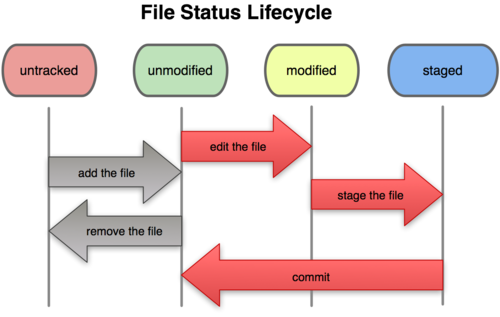
\includegraphics[scale=0.7]{Status_lifecycle.png}
    \end{center}
    \tiny
    \caption{cc progit.org}
    \label{cc progit.org}
  \end{figure}
\end{frame}

\section{Installer et configurer Git}

\subsection*{Installation}
\begin{frame}{Installation}
\end{frame}

\subsection*{Configuration}
\begin{frame}{Configuration}
\end{frame}

\section{Les Bases de Git}
\begin{frame}{Les Bases de Git}
  \begin{itemize}
    \item Créer un dépot : 
    \item Cloner un dépot :
  \end{itemize}
  
\end{frame}

\section{Le Branching}
\begin{frame}{}
\end{frame}

\section{Utilisation Avancée}
\begin{frame}{}
\end{frame}

\section{Ressources}
\begin{frame}{}
  \begin{itemize}
    \item \href{http://progit.org/about.html}{Progit}
    \item \href{http://git.or.cz/gitwiki/GitHosting}{Liste de serveurs Git}

  \end{itemize}
\end{frame}

\end{document}
